\documentclass[]{auvsi_doc}
\setkeys{auvsi_doc.cls}{
	AUVSITitle={Airframe Concept Description},
	AUVSILogoPath={./figs/logo.pdf}
}

% include extra packages, if needed

\begin{document}

\begin{AUVSITitlePage}
\begin{artifacttable}
\entry{AF-002, 0.1, 10-31-18, Initial Draft, Tyler Critchfield, Ryan Anderson}
\entry{AF-002, 0.2, 11-06-18, Revisions for Final Submission, Tyler Critchfield, [CHECKED BY]}
% additional \entry{} commands for extra rows in the revision table, if needed
\end{artifacttable}
\end{AUVSITitlePage}

\section{Introduction}

This artifact describes our chosen airframe concept and how it relates to our key success measures.

\section{Concept Description}

We selected the modified Nimbus Pro as our chosen concept for the Airframe subsystem. This airframe modifies a traditional twin propulsion fixed wing RC airframe (see Figure \ref{fig:nimbus}) that can be purchased off the shelf. The original RC airframe has a wing span of 1.95m, a wing area of 5700 cm$^2$, a fuselage length of 1.29m, a payload storage volume of about 8000 cm$^3$, and an empty weight of 1.9 kg. In this design, about two-thirds of the wings are able to be disconnected for easy storage and transport (see Figure \ref{fig:wing}). We could use this to our advantage and create new wing extensions to attach to the plane instead of the original wings. These wing extensions would likely have a longer span, but would be restricted to the existing design in root airfoil shape and root chord length. We would have freedom to adjust span, taper ratio, tip twist, and a tip airfoil if we so choose. We would model these design parameters in XFLR5 to determine the best wing extension design. The wing extensions would be made of foam and easily constructed using the foam cutter in EB 112. The modular nature of these adjustments would make it easy to assemble and rebuild if necessary, especially if redundant parts are purchased and created. This is critical to our team's success this year. To be successful, each subsystem will need to prototype and test their designs often - but no one can truly test their designs without an airframe that flies. Having a modular wing design would still allow for fast rebuild, ensuring that other team members would not be wasting time waiting for a new plane to be built. In the case that a redesign is necessary, the other subsystem teams can use the existing wings for the Nimbus Pro while waiting. Or in the case that the performance of these design modifications does not justify the extra time and effort, the original Nimbus Pro design will still work and not require adaptation to implement.

\section{Key Success Measures}

This airframe concept was selected to best achieve our key success measures, which in turn will help us maximize our competition performance. Specifically, we needed an airframe that could fly at a slower velocity and had more storage capacity to hold our UGV (Unmanned Ground Vehicle) payload. A slower velocity will assist the autopilot to plan and execute a flight path that minimizes obstacles hit, waypoint proximity, and manual takeovers required - three of our key success measures. In addition, a slower velocity will result in better image quality from our camera, which will increase the percentage of characteristics identified by the imaging team. A slower velocity will also help airdrop accuracy. 
Payload storage capacity will prevent us from needing to mount the payload to the airframe exterior. Keeping the payload inside the airframe will prevent excess drag and allow the plane to fly at a slower velocity, assisting all of the key success measures already mentioned. In addition, the time to build the airframe was another measure we used to select our chosen concept that indirectly affects all of the key success measures. If the airframe takes too long to build, it is difficult for us to test our other subsystems that are directly working on those key success measures (e.g. imaging subsystem needing to test identified characterisitcs). We are confident the Modified Nimbus Pro concept will help us maximize our performance in the key success measures.

\begin{figure}[h!]
	\centering
	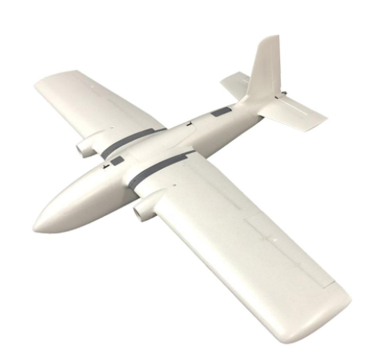
\includegraphics[scale=0.7]{figs/NimbusPro}
	\caption{The Nimbus Pro from My Fly Dream. Image taken from banggood.com.}
	\label{fig:nimbus}    
\end{figure}

\begin{figure}[h!]
	\centering
	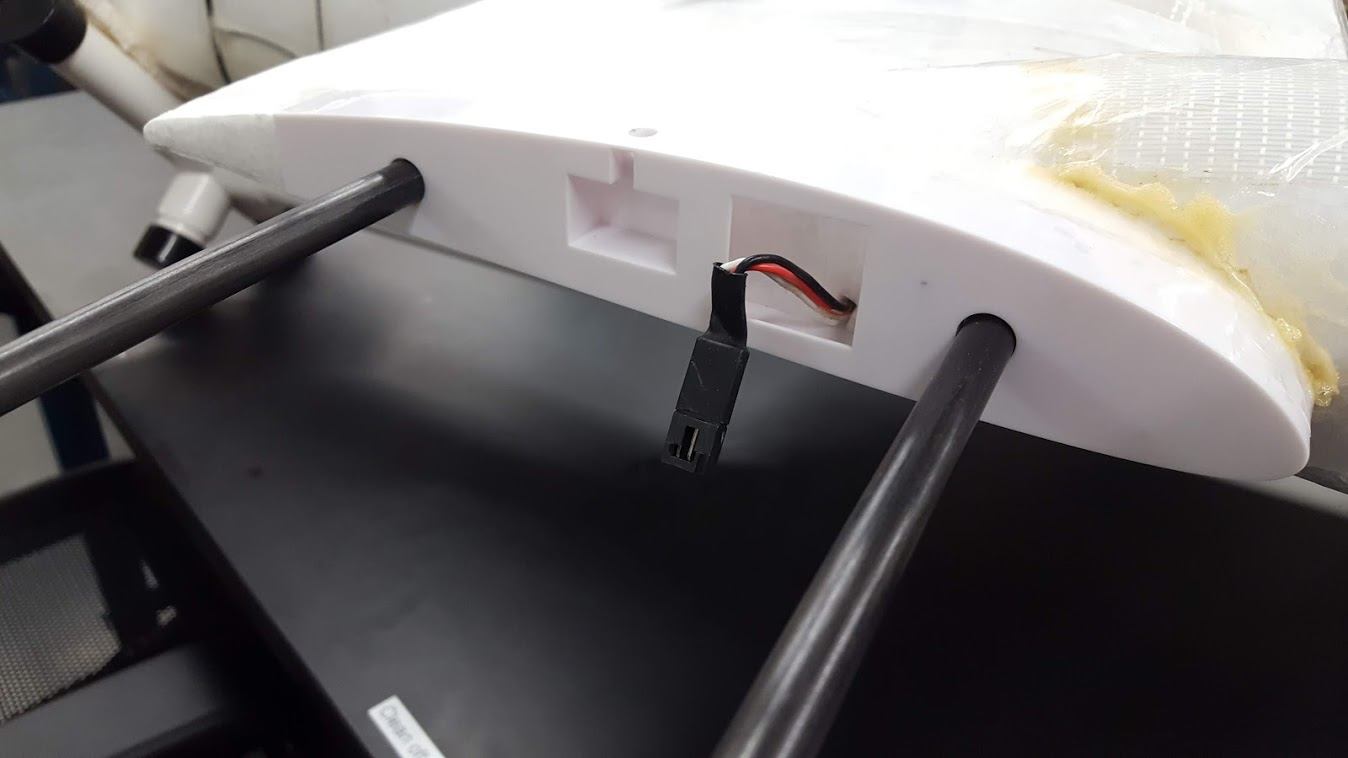
\includegraphics[width=.8\columnwidth]{figs/wing}
	\caption{This is where the wing disassembles and where we would attach our custom wings. This is a photo of My Twin Dream, but this concept is the same for the Nimbus Pro.}
	\label{fig:wing}    
\end{figure}

\end{document}